\documentclass[a4paper,10pt,twoside, top=3.3cm,
bottom=4.2cm, left=2.6cm, right=2.6cm]{article}
%,columnsep=5cm

\usepackage{epsfig}
\usepackage{subfigure}
\usepackage{calc}
\usepackage{amssymb}
\usepackage{amstext}
\usepackage{amsmath}
\usepackage{amsthm}
\usepackage{multicol}
\usepackage{pslatex}
\usepackage{apalike}
\usepackage{SCITEPRESS}
\usepackage[small]{caption}

%\usepackage[twocolumn,textwidth=15.8cm,columnsep=.8cm]{geometry}

%\let\oldtabular\tabular
%\renewcommand{\tabular}{\small\oldtabular}

\subfigtopskip=0pt
\subfigcapskip=0pt
\subfigbottomskip=0pt

%\usepackage{url}
\usepackage[utf8]{inputenc}

\usepackage{array}

\usepackage{tikz}
\usepackage{pgfplots}

%\newcommand{\keywords}[1]{\par\addvspace\baselineskip
%\noindent\keywordname\enspace\ignorespaces#1}

\renewcommand{\textfraction}{0}
\renewcommand{\topfraction}{1}
\renewcommand{\bottomfraction}{1}
\renewcommand{\floatpagefraction}{0.9}

\newcommand{\simpleEntry}[1]{
\vspace{.3cm}
\noindent \textbf{#1}
\vspace{.3cm}
}

\usepackage{listings}
\lstdefinelanguage{scala}{
  morekeywords={abstract,case,catch,class,def,%
    do,else,extends,false,final,finally,%
    for,if,implicit,import,match,mixin,%
    new,null,object,override,package,%
    private,protected,requires,return,sealed,%
    super,this,throw,trait,true,try,%
    type,val,var,while,with,yield},
  otherkeywords={=>,<-,<\%,<:,>:,\#,@},
  sensitive=true,
  morecomment=[l]{//},
  morecomment=[n]{/*}{*/},
  morestring=[b]",
  morestring=[b]',
  morestring=[b]"""
} % from stackoverflow

\usepackage{fancyvrb}
\usepackage{framed}
%\usepackage[listings,skins]{tcolorbox}
\usepackage[skipbelow=\topskip,skipabove=\topskip]{mdframed}
\mdfsetup{roundcorner=0}

\hyphenation{experimentRun}

%\author{A. N. Onymous ~\inst{Anonymity institution, http://anonymi.ty}}

%\authorrunning{J. Albert Cruz et al.}
%\institute{Centro de Estudios de Matem\'atica Computacional, Universidad de Ciencias Inform\'aticas, Cuba
%\and Dept. Arquitectura y Tecnología de los Computadores, Universidad de Granada, España \\
%jalbert@uci.cu}


%\tocauthor{Authors' Instructions}


\begin{document}

\title{Implementing Parallel Genetic Algorithm Using Concurrent-Functional Languages}

%\author{J. Albert-Cruz\inst{1}, J.J. Merelo\inst{2}, L. Acevedo-Martínez\inst{1}, Paloma de las Cuevas \inst{2}}
%
%\author{\IEEEauthorblockN{J. Albert-Cruz\IEEEauthorrefmark{1}, J.J. Merelo\IEEEauthorrefmark{2}, L. Acevedo-Martínez\IEEEauthorrefmark{1} and Paloma de las Cuevas\IEEEauthorrefmark{2}}\\
%\IEEEauthorblockA{\IEEEauthorrefmark{1}Centro de Estudios de Matem\'atica Computacional, Universidad de Ciencias Inform\'aticas, Cuba\\
%Email: \{jalbert,liesner\}@uci.cu}\\
%\IEEEauthorblockA{\IEEEauthorrefmark{2}Dept. Arquitectura y Tecnología de los Computadores, Universidad de Granada, España\\
%Email: \{jmerelo,paloma\}@geneura.ugr.es}
%}


%\author{
%\authorname{A. N. Onymous\sup{1}}
%\affiliation{\sup{1}Anonymity institution, http://anonymi.ty}
%\email{onymous@anonymi.ty}
%}

\author{\authorname{J. Albert-Cruz\sup{1}, J.J. Merelo\sup{2}, L. Acevedo-Martínez\sup{1}, and Paloma de las Cuevas\sup{2}}
\affiliation{\sup{1}Centro de Estudios de Matem\'atica Computacional, Universidad de Ciencias Inform\'aticas, Cuba}
\affiliation{\sup{2}Dept. Arquitectura y Tecnología de los Computadores, Universidad de Granada, España}
\email{\{jalbert,liesner\}@uci.cu, \{jmerelo,paloma\}@geneura.ugr.es}
}


\keywords{Parallel Evolutionary Algorithms, Functional Languages, Concurrent Languages, Implementation, Modeling.}


\abstract{The spread of multiprocessor and multi-core architectures have a
pervasive effect on the way software is developed. In order to take
full advantage of them, a parallel implementation of every single
program would be needed, but also a radical reformulation of the
algorithms that are more appropriate to that kind of implementation. In this work we design and implement an evolutionary
computation model using programming languages with built-in concurrent
concepts. This article shows the advantages of these paradigms in
order to implement a  parallel genetic algorithm (pGA) with an island
pools based topology in the concurrent-functional oriented programming
languages: Erlang, Scala, and Clojure. Some implementation decisions
are analyzed and the results of the solution of a study case are
shown.}

\onecolumn \maketitle \normalsize \vfill

\section{\uppercase{Introduction}}
\label{sec:intro}
    
\noindent Genetic algorithms (GA) are currently one of the most used meta-heuristics to solve Computer Science problems. They can obtain solutions to complex optimizations problems in adequate times \cite{Luque2011}. These algorithms consists in evolving sets of individuals (populations), as it is on nature, to find or improve a solution to a problem.

Parallel genetic algorithms (pGAs) are GAs in which the possible solutions are evaluated or the process of evolution is made in parallel. That kind of behavior is specially good for problems with expensive exploration of the search space; some researchers are found also \cite{Alba2001}, with the different search process, it’s improve the quality of solutions.

%La segunda frase del párrafo anterior no tiene sentido, no sé qué se quiere decir.
%Lo mismo con la primera frase del siguiente párrafo, hasta la coma.

The field is feature rich, several models have been created and new kind of problems are have been tried to solve, nevertheless the programming paradigm used in the implementation of such algorithms is far from being an object of study. Technologies like Java and C/C++ are mostly used, and, although some think that implementation matters \cite{DBLP:conf/iwann/MereloRACML11}, is not much the research that the community do approaching to new programming languages/paradigms.

%Del último párrafo, desde "isn't much the..." en la última frase, no tiene sentido.

The multicore’s challenge \cite{SutterL05} is a current need for making parallel even the simplest program. But this way leads us to use and create design patterns for parallel algorithms; the conversion of a pattern into a language feature is a common practice in the programming languages domain, and sometimes that’s means a language modification, others the creation of a new one.

This work explores the advantages of some non mainstream languages with concurrent and functional features in order to develop pGAs. It is motivated by the lack of community attention on the subject and the belief that using concepts that simplify the modeling and implementation of such algorithms it might promote their use in research (achieving a paradigm shift to create more efficient algorithms) and in practice (for being the implementations of the parallels variants very simple). We are continuing the research reported in \cite{DBLP:conf/gecco/CruzGGC13,J.Albert-Cruz2013} and we are trying to find the better options.

%El resto del trabajo se estructura como sigue: introducción y motivación (Sección \ref{sec:intro}), paradigmas y lenguajes multiparadigmas dentro del que se caracterizan los lenguajes funcionales y concurrentes (Sección \ref{sec:paradigmas}) así como algunos lenguajes emergentes (Sección \ref{sec:emergentes}). A continuación se muestra la modelación e implementación de un algoritmo genético usando conceptos de los paradigmas antes expuestos (secciones \ref{sec:design} y \ref{sec:impl}); y finalmente, se presentan los resultados (Sección \ref{sec:results}) y conclusiones (Sección \ref{sec:conclusions}).


\section{\uppercase{Functional and concurrent programming}}
\label{sec:stateArt}
\noindent Developing correct software quickly and efficiently is a never ending goal in the software industry. Novel solutions that try to make a difference providing new abstraction tools outside the mainstream of programming languages have been proposed to pursue this goal; two of the most promising are the functional and the concurrent.

%-------------------------------------------------------------------------------------------------------------------------------------------------------

%\simpleEntry{Paradigms}
%\label{sec:paradigmas}


%Functional languages have been available for a long time, in the shape of LISP, which was introduced in the fifties, nevertheless their use has been limited mainly due to the inefficiency of their compilers or interpreters. Currently these situations have changed, the problems with efficiency are solved and their newly found advantages have promoted the inclusions of several functional concepts in modern and mainstream languages. C\# for example, or even the creation of new ones such as Clojure, which excels among the emergent languages with the concurrent paradigm together with Go, Scala, Haskell and Erlang \cite{DiPierro:2012:CMP}; they have built-in programming constructs for managing concurrency simplifying its use.

\simpleEntry{Concurrent programming}
    
The concurrent programming paradigm (or concurrent oriented programming \cite{Armstrong2003}) is characterized by the presence of programming constructs for manage process like first class objects. That’s with operators for act upon them and the possibility of using it like parameters or function's result values.

Concurrent programming is hard for many reasons, the communication between processes is central in the design of such algorithms. One of the best efforts to formalize and simplify that is the Hoare’s {\em Communicating Sequential Processes} \cite{Hoare:1978:CSP:359576.359585}, this interaction description language are the theorical support for many libraries  and new programming languages. 

\simpleEntry{Functional programming}
    El paradigma de la programación funcional por su parte, aún cuando ofrece varias ventajas, no ha sido muy usado. Un tiempo atrás se exploraron en el campo de la Programación Genética \cite{Briggs:2008:FGP:1375341.1375345,Huelsbergen:1996:TSE:1595536.1595579,walsh:1999:AFSFESIHLP}, más recientemente en la neuroevolución  \cite{Sher2013}; sin embargo dentro de los AG ha sido poca su presencia \cite{Hawkins:2001:GFG:872017.872197}.

La programación funcional se caracteriza por el uso de las funciones como datos (pasándolas por parámetros y devolviéndolas como resultados), en particular de las funciones puras: aquellas cuyo resultado solo depende de los parámetros de entrada, excluyendo los cambios de estado. Esto la hace particularmente adecuada para el desarrollo de algoritmos concurrentes pues estos tienen la primera fuente de errores y complejidad en la comunicación entre procesos, a través de cambios de estado.

El uso de listas, con implementaciones muy eficientes, es omnipresente en la programación funcional; en los AGs por su parte es una de las estructuras de datos más utilizadas, lo cual facilita el proceso de implementación de los diversos modelos de algoritmos evolutivos.



\simpleEntry{Multi-paradigm emerging languages} %emerging
    
The field of programming languages research is very active in the Computer Science discipline. To find software construction tools with new and better means of algorithms expression is well welcome. In the last few years the functional and concurrent paradigms have been produced a rich mix in which concepts of the first one had been simplified the use of the second one.

%Esta sección es un poco corta...

\section{\uppercase{A concurrent and functional approach to pGAs}}
\label{sec:design}
    \subsection{Caso de estudio}

Para lograr una buena implementación de un algoritmo es necesario tener en cuenta las características del lenguaje en el que se realizará así como cada concepto constituyente del dominio del problema. Se usará como caso de estudio un AG paralelo híbrido, sobre una topología de isla (ver Figura \ref{fig:topologia}), en la que cada nodo será a su vez un AG concurrente basado en pool.

El problema a utilizar será el {\em SAT-MAX} con instancias de 100 variables tomadas de \cite{Hoos2000}.

%
%\subsection{Caso de estudio}
%
%El objetivo de este trabajo es validar las facilidades de Erlang para implementar AGs, por ello hemos tomado un problema muy sencillo ({\em OneMax}): el simple conteo del número de unos en una cadena binaria, siendo la solución óptima la alcanzada cuando coincide la longitud de la lista con dicha cantidad. Dadas las características de la arquitectura diseñada y la posibilidad de correr nodos Erlang en disímiles dispositivos, la adaptación de este trabajo a otros problemas más complejos solamente requeriría redefinir las funciones de evaluación, cruce y mutación.

\subsection{Arquitectura}

Los componentes del AG paralelo identificados como principales a la hora de diseñar la implementación aparecen listados en la Tabla \ref{agpComp}. Las construcciones de Erlang utilizadas para la modelación son las expuestas en la Tabla \ref{erlComp} y el mapeo realizado es el mostrado en la Tabla \ref{erlAGRelation}.


\begin{table}
  \centering
  \caption{Componentes del AG paralelo.}\label{agpComp}
   \begin{tabular}{|p{3cm}|p{5cm}|p{3cm}|}
   \hline
   \textbf{Componente AG} & \textbf{Papel} & \textbf{Descripción}\\
     \hline
      cromosoma & Representación de la solución al problema. & cadena binaria \\
     \hline
      cromosoma evaluado & Par \{cromosoma, fitness\}. & cantidad de valores 1\\
     \hline
      población & Conjunto de cromosomas. & lista\\
     \hline
     cruzamiento & Relación entre dos cromosomas que da por resultado otros dos nuevos. & función de cruzamiento\\
     \hline
      mutación & Modificación de un cromosoma.& función que altera un valor\\
     \hline
     selección & Criterio para obtener una sublista a partir de la población. & función de selección\\
     \hline
      pool & Población compartida entre las unidades de cálculo en un nodo. & población\\
     \hline
      isla & Nodo de la topología. & población\\
     \hline
      migración & Evento aleatorio de intercambio de cromosomas. & mensaje\\
     \hline
   \end{tabular}

\end{table}


\subsection{Modeling and Implementing in Concurrent Languages}
\label{sec:impl}
    
With the initial domain analysis and using the concurrent and functional concepts properly, the following design and implementation were conceived. 

\simpleEntry{Erlang modeling}
    
The main concurrent concepts are actor and message; the functional concepts are function and list. It was used actors (the executing units of the language) for the independent process: islands or evaluators/reproducers. The communication among them was made by messages, that’s the concept available in the pattern.

GA’s logic was expressed by functions, the functional means for data transformation and computation expression, and the data model was coded using lists and tuples: the basics data structures in the functional paradigm.


\begin{table}[h!]
  \centering
   \caption{Erlang's constructions.}\label{erlConstructions}
\begin{tabular}{|>{\centering}p{3.4cm}|p{7cm}|}
  \hline
  % after \tabularnewline: \hline or \cline{col1-col2} \cline{col3-col4} ...
  \textbf{Erlang's Concept} & \textbf{Role} \tabularnewline
     \hline
  tuple & Data structure for immutable compound data. \tabularnewline
     \hline
  list & Sequence data structure for variable length compound data. \tabularnewline
     \hline
  function & Data's relations, operations. \tabularnewline
     \hline
  actor & Executing unit, process. \tabularnewline
     \hline
  message & Communication among actors. \tabularnewline
     \hline
  {\em ets} & Set of chromosome shared by the pool. \tabularnewline
     \hline
  {\em random} module& Random number generation. \tabularnewline
  \hline
\end{tabular}

\end{table}

\begin{table}
  \centering
  \caption{Erlang/AG's concepts mapping.}\label{erlAGRelation}
\begin{tabular}{|>{\centering}p{3cm}|p{6cm}|}
  \hline
  \textbf{Erlang concept} & \textbf{AG concept mapping} \tabularnewline
     \hline
  tuple & evaluated chromosome \tabularnewline
     \hline
  list & chromosomes and populations \tabularnewline
     \hline
  function & crossover, mutation and selection \tabularnewline
     \hline
  actor  & island, evaluator and reproducer \tabularnewline
     \hline
  message & migration \tabularnewline
     \hline
  {\em ets}  & pool \tabularnewline
     \hline

\end{tabular}

\end{table}




%\simpleEntry{Library erlEA}
%    En la realización del caso de estudio fue implementado, teniendo en cuenta los conceptos seleccionados anteriormente, un proyecto Erlang de varios módulos. El código se encuentra bajo la licencia AGPL, de código abierto, en la dirección: \url{https://github.com/jalbertcruz/erlEA/tree/book2013}. Sus principales módulos y funciones son descritos a continuación.


\subsubsection{Módulo reproducer}

Este es el módulo que selecciona la subpoblación a reproducir, los padres, realiza el cruzamiento y desencadena las migraciones. Como actor responde a los mensajes {\em evolve}: para realizar una iteración y {\em emigrateBest} para efectuar una emigración. Las funciones con las que logra esto aparecen enumeradas en la Tabla \ref{tb:reproducer}.

\begin{table}
  \caption{Funciones del módulo reproducer.}\label{tb:reproducer}
  \centering
\begin{tabular}{|p{5cm}|p{7cm}|}
  \hline
  % after \\: \hline or \cline{col1-col2} \cline{col3-col4} ...
   \textbf{Función} &  \textbf{Descripción} \\
  \hline
  {\tt extractSubpopulation(Table, N) } & A partir de una {\em ets} y una cantidad, selecciona de la {\em ets} un grupo de cromosomas. \\
  \hline
  {\tt bestParent(Pop2r)} & Selecciona de una lista de cromosomas el mejor individuo. \\
  \hline
 {\tt selectPop2Reproduce(Pop, N)} & Selecciona aleatoriamente un conjunto de pares de una lista de cromosomas. \\
  \hline
  {\tt crossover(Ind1, Ind2)} & Realización de un cruce y mutación sobre el mismo, a partir de dos cromosomas. \\
  \hline
\end{tabular}
\end{table}


\subsubsection{Módulo evaluator}

Este es el módulo que calcula el fitness: hace periódicas consultas sobre el pool para obtener individuos a los que calcularle el fitness. Está compuesto por la función {\em SatMax/1} (función de evaluación), y por el mensaje {\em eval}, dicho mensaje es el que activa al evaluador para que calcule.

\subsubsection{Módulo poolManager}

Este es el módulo encargado de inicializar el trabajo del pool así como enrutar los mensajes entre los evaluadores. Es el encargado de controlar la finalización del algoritmo una vez se ha encontrado la solución.  Los mensajes a los que responde este actor aparecen enumerados en la Tabla \ref{tb:poolManager}.

\begin{table}
  \caption{Mensajes a los que responde el actor del módulo poolManager.}\label{tb:poolManager}
  \centering
\begin{tabular}{|p{3cm}|p{7cm}|}
  \hline
  % after \\: \hline or \cline{col1-col2} \cline{col3-col4} ...
   \textbf{Mensaje} &  \textbf{Descripción} \\
  \hline
  {\tt evolveDone } & Finalización de una iteración de reproducción. \\
  \hline
  {\tt evalDone} & Finalización de una iteración de evaluación. \\
  \hline
 {\tt solutionReached} & Obtención de la solución. \\
  \hline
  {\tt migration} & Realización de una inmigración. \\
  \hline
\end{tabular}
\end{table}


\subsubsection{Módulos auxiliares e interconexión}

Los módulos ya descritos contienen toda la lógica del AG, faltan sin embargo, para que sea operativo el software, algunos componentes no funcionales.

\vspace{.35cm}

\noindent  Dichos componentes son:
\begin{description}

  \item[experiment] -- Encargado de iniciar una corrida del experimento.

  \item[configBuilder] -- Especificación de los parámetros de un experimento.

  \item[profiler] -- Análisis del comportamiento: tiempos de ejecución, cantidad de iteraciones, etc.

  \item[manager] -- Control del inicio y coordinación de la finalización adecuada de cada unidad de ejecución durante la corrida de un experimento.

  \item[report] -- Control de la secuencia de experimentos y emisión del reporte final resultado de la experimentación.

\end{description}

\noindent Los diferentes módulos interactúan de la siguiente manera durante una sesión de experimentación:

\begin{enumerate}

  \item Configuración de los parámetros: tamaño de población y cromosomas, población inicial, conformación de la topología de las islas. Módulos {\em experiment} y {\em configBuilder}.

  \item Lógica del AG: reproducción, selección de padres, emigraciones, cálculo del fitness. Módulos {\em evaluator} y {\em reproducer}.

  \item Control del proceso y reportes: enruteo de mensajes entre islas y unidades de ejecución (actores), coordinación de los procesos de finalización de una corrida e inicio de otra, resumen y formateo de salida de los resultados. Módulos {\em poolManager}, {\em profiler}, {\em manager} y {\em report}.

\end{enumerate}



\simpleEntry{Scala modeling}
    
Scala is a programming language with the same concurrent programming pattern (actors) than Erlang. In the Scala implementation we followed the same criteria like in Erlang but with differences for its object support and JVM dependence.

%Las tablas no están referenciadas

\begin{table}[h!]
  \centering
   \caption{Scala's concepts.}\label{sclConstructions}
\begin{tabular}{|>{\centering}p{3.4cm}|p{7cm}|}
  \hline
  % after \tabularnewline: \hline or \cline{col1-col2} \cline{col3-col4} ...
  \textbf{Scala's concepts} & \textbf{Role} \tabularnewline
  tuple & Data structure for immutable compound data. \tabularnewline
    \hline
 list & Sequence data structure for variable length compound data.
 \tabularnewline
    \hline
 function & Data's relations, operations. \tabularnewline
     \hline
    Akka's actor & Executing unit, process. \tabularnewline
     \hline
  symbol/message & Communication among actors. \tabularnewline
     \hline
  {\em HashMap} & Set of chromosome shared by the pool. \tabularnewline
     \hline
\end{tabular}

\end{table}

\begin{table}
  \centering
  \caption{Scala/AG's concepts mapping.}\label{sclAGRelation}
\begin{tabular}{|>{\centering}p{3cm}|p{6cm}|}
  \hline
  \textbf{Scala concept} & \textbf{AG concept mapping} \tabularnewline
  \hline
   tuple & evaluated chromosome \tabularnewline
    \hline
 list & chromosomes and populations \tabularnewline
    \hline
 function & crossover, mutation and selection \tabularnewline
    \hline
  Akka's actor & island, evaluator and reproducer \tabularnewline
     \hline
  symbol/message & migration \tabularnewline
     \hline
  {\em HashMap} & pool \tabularnewline
     \hline
\end{tabular}

\end{table}








%\simpleEntry{Library sclEA}
%    
We developed a library in Scala following the same design concepts and it was tested with the case study. The code is open, under AGPL license, at \url{https://github.com/jalbertcruz/sclEA/archive/v1.0.tar.gz}. The main classes and objects are briefly described.

\subsubsection{Evaluator/Reproducer's classes}

The reproducer class select the subpopulation and parents for reproduction, it does the crossover and activate migrations. As actor respond to {\em evolve} and {\em emigrateBest} messages, for iteration and migration operations.

Class {\em Evaluator} consults the pool constantly looking for no-evaluated individuals. It is compound by the function {\em evaluate/1} (general evaluation function), and the message: {\em evaluate} for fire the calculation.

These two kinds of actors are the execution units working to reach the solutions. They have, concerning architecture, the same role as Erlang’s actors, with the same behavior but in an object oriented way.


\simpleEntry{Clojure modeling}
    
The Clojure’s main concurrent used concepts are \textbf{agent}, \textbf{ref} and \textbf{atom}; the functional ones are \textbf{function} and \textbf{list}. Clojure is a language with a very strict control of state changes; it demands a clear identification of the code doing it % Haciendo qué?
 and that is similar to Erlang where the functional purity is pursued too.

Agents were the concept used for implementing the independent units of execution (reproductors, evaluators, and islands). The communication between agents was made by protocol’s functions due to the needed flexibility. GA’s operations, their logic and constraints, were expressed in functions and protocol implementations and the data was encoded in lists and vectors data structures. 

%\simpleEntry{Library cljEA}
%    
We developed a library in Clojure following the same design concepts and it was test with the case study. The code is open, under AGPL license, at \url{https://github.com/jalbertcruz/cljEA/tree/evostar2014}. In this implementation are used the same naming and architectural convection than with Erlang and Scala.
%

\simpleEntry{Libraries developed}
    
We developed libraries in Erlang, Scala and Clojure following the same design concepts and it was tested with the study case. The code is open, under AGPL license, at the following addresses:

\begin{description}
  \item[Erlang] \url{https://github.com/jalbertcruz/erlEA/archive/v1.0.tar.gz}
  \item[Scala] \url{https://github.com/jalbertcruz/sclEA/archive/v1.0.tar.gz}
  \item[Clojure] \url{https://github.com/jalbertcruz/cljEA/archive/v1.0.tar.gz}
\end{description}


\subsection{Application Over the Study Case} \label{sec:results}%Application over the study case
    
All used languages have functional and concurrent built-in features, with the first ones supporting the second ones. Erlang and Scala’s implementations are based in the actor pattern for doing parallel computation. Clojure on the other hand works with the agent concept, a similar model with simplified ways of reading the involved information.

To communicate modules we used language’s dependent (and different) data types.
The message's structure was tuples for Erlang and Scala, and for agents it was necessary to encapsulate functions on protocols (Clojure variants of Java interfaces). For sharing individuals (the pool) we used functionals consult/modification data structures: hash-like for Scala/Clojure and the {\em ets} module in Erlang’s case. The data was encoded with compound data structures: lists, vectors, tuples, records, etc. The Table \ref{tb:res:comp} summarizes the differences between the languages.

\begin{table*}\small
  \caption{Language concept used for each pGA component.}\label{tb:res:comp}
  \centering
%\begin{tabular}{|p{2.2cm}|>{\centering}p{1.6cm}|>{\centering}p{1.6cm}|>{\centering}p{1.8cm}|}
  \begin{tabular}{|>{\centering\arraybackslash}p{4cm}|>{\centering\arraybackslash}p{2.4cm}|>{\centering\arraybackslash}p{2.4cm}|>{\centering\arraybackslash}p{3cm}|}    \hline
     & \textbf{Erlang} & \textbf{Scala} & \textbf{Clojure} \tabularnewline
    \hline
    Parallel execution unit & actor & actor & agent \tabularnewline
    \hline
    Communication (messages) & tuple & tuple & function (protocol) \tabularnewline
    \hline
    pool & \emph{ets} & HashMap & hash-map \tabularnewline
    \hline
    DS chromosome & list & list & vector \tabularnewline
    \hline
    DS population & list & list & lazy list \tabularnewline
    \hline
    Compound data & tuple & tuple/object & record/vector \tabularnewline
    \hline
    Runtime environment & Erlang VM & Java VM & Java VM \tabularnewline
    \hline
  \end{tabular}

\end{table*}


\simpleEntry{Results}

The design was tested with a population of 1024 individuals on each island (two islands were used), doing 5000 evaluations on a dual-core (4 threads) laptop  i7-3520M with Windows 8 and 16 Gb of RAM. In order to find the better combinations of evaluators/reproducers, several of them were tested for each technology (evaluators = $1..30$ and reproducers = $1..10$). In every combination the number of evaluators is greater than the reproducers because the fitness function is more computational intensive than the reproduction execution. 10 runs were used for each combination and then the times with more dispersion were deleted until the standard deviation (SD) remained below the 5 \%.

For a \emph{speedup} analysis, using the ideas presented in \cite{Alba02parallelevolutionary},  a sequential implementation with the same data structures and operator's implementations was made. Speedup is the ratio between $E[T_1]$ (sequential implementation average time) and $E[T_m]$ (parallel implementation average time in $m$ processors), the expected value is $m=4$ in this case (the number of logical processors in the used hardware).

\begin{table*}\small
  \caption{Experiment results for the minimum parallel time of all combinations tested.}\label{tb:resAll}
  \centering
%\begin{tabular}{|>{\centering}p{.85cm}|>{\centering}p{1.4cm}|
%>{\centering}p{1.4cm}|>{\centering}p{.9cm}|>{\centering}p{1cm}|
%>{\centering}p{.8cm}|>{\centering}p{.45cm}|}
\begin{tabular}{|>{\centering\arraybackslash}p{1.6cm}|>{\centering\arraybackslash}p{2.5cm}|
>{\centering\arraybackslash}p{2.4cm}|>{\centering\arraybackslash}p{2.1cm}|>{\centering\arraybackslash}p{1.7cm}|
>{\centering\arraybackslash}p{1.45cm}|>{\centering\arraybackslash}p{1.45cm}|}

  \hline
  \textbf{Language} & \textbf{Parallel time $\pm$ SD (ms)} & \textbf{Workers combination} & \textbf{Sequential time (ms)} & \textbf{Relative speedup} & \textbf{Speedup}\tabularnewline
  \hline
  Erlang & 2920.40 $\pm$ 126 & 25 evaluators, 1 reproducer & 8143.3 & 2.78 & 0.55 \tabularnewline
  \hline
  Clojure & 1734.66 $\pm$ 28.32 & 10 evaluators, 1 reproducer & 3340.22 & 1.92 & 0.92 \tabularnewline
  \hline
  Scala & 563 $\pm$ 24.32 & 6 evaluators, 1 reproducer & 1651.8 & 2.86 & 2.86 \tabularnewline
  \hline
\end{tabular}
\end{table*}

The results shown in Table \ref{tb:resAll} indicate for each language the best time for the parallel implementation, the combination of evaluators/reproducers in which the parallel variant was obtained, the time for the sequential implementation, a relative speedup (speedup calculated in relation to his sequential time) and the speedup (relative to the best sequential time of all implementations, Scala's in this case). Each worker (evaluators and reproducers) is a unit of execution, and in the used hardware only 4 units (at most) can run at the same time.

Figure 1 shows the running times when one reproducer is used with a variant number of evaluators;  Figure 2 shows the same but for two reproducers. In both cases the overall behaviour of Scala is better. The computation complexity of the evaluation function is greater than the reproduction phase and this is why the results when one reproducer was used are better than when two reproducers were used.

%\begin{small}
%\begin{itemize}
%
%\item[] 
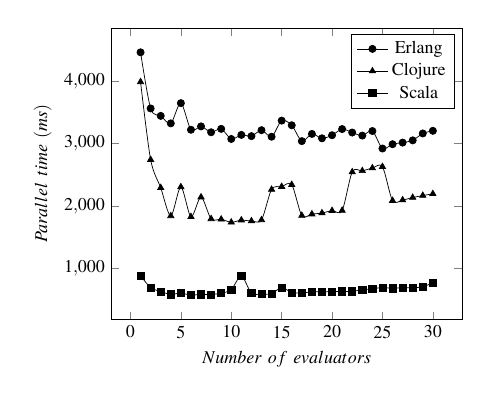
\begin{tikzpicture}[thick, scale=0.65]

  \begin{axis}[
         xlabel=$Number \hspace{.12cm} of \hspace{.12cm} evaluators$,
         ylabel=$Parallel \hspace{.12cm} time \hspace{.12cm} (ms)$
         ]
     \addplot[smooth,mark=*]  plot coordinates{
(1,4466.6)
(2,3564.222222222222)
(3,3444.6666666666665)
(4,3324.5555555555557)
(5,3649.6)
(6,3221.7)
(7,3275.9)
(8,3181.3)
(9,3236.0)
(10,3073.5555555555557)
(11,3139.0)
(12,3119.1111111111113)
(13,3214.9)
(14,3109.5555555555557)
(15,3368.3)
(16,3293.7)
(17,3039.1)
(18,3154.7)
(19,3084.1)
(20,3133.6666666666665)
(21,3232.9)
(22,3177.1111111111113)
(23,3128.0)
(24,3201.3333333333335)
(25,2920.4)
(26,2989.5555555555557)
(27,3015.4)
(28,3051.4444444444443)
(29,3162.3)
(30,3204.7)
     };
     \addlegendentry{Erlang}

     \addplot[smooth,mark=triangle*]
         plot coordinates{
(1,3990.75)
(2,2740.777777777778)
(3,2289.1111111111113)
(4,1837.111111111111)
(5,2302.5555555555557)
(6,1822.6666666666667)
(7,2138.6666666666665)
(8,1789.5)
(9,1782.3333333333333)
(10,1734.6666666666667)
(11,1768.888888888889)
(12,1754.7777777777778)
(13,1772.0)
(14,2261.1111111111113)
(15,2307.8888888888887)
(16,2338.4444444444443)
(17,1842.3333333333333)
(18,1865.7777777777778)
(19,1883.4444444444443)
(20,1920.7777777777778)
(21,1923.5)
(22,2542.1111111111113)
(23,2561.6666666666665)
(24,2605.5555555555557)
(25,2627.0)
(26,2083.0)
(27,2091.8888888888887)
(28,2132.222222222222)
(29,2163.777777777778)
(30,2192.1111111111113)
         };
     \addlegendentry{Clojure}


     \addplot[smooth,mark=square*]
         plot coordinates{
(1,876.6666666666666)
(2,683.7777777777778)
(3,622.2857142857143)
(4,575.2222222222222)
(5,596.0)
(6,563.0)
(7,576.2222222222222)
(8,574.0)
(9,595.1111111111111)
(10,651.8888888888889)
(11,871.6666666666666)
(12,595.3333333333334)
(13,582.25)
(14,586.8888888888889)
(15,684.8888888888889)
(16,605.0)
(17,600.625)
(18,614.0)
(19,618.2222222222222)
(20,616.7777777777778)
(21,625.2222222222222)
(22,622.6666666666666)
(23,649.7777777777778)
(24,664.1111111111111)
(25,686.625)
(26,672.4444444444445)
(27,684.7777777777778)
(28,681.625)
(29,698.0)
(30,760.7142857142857)
         };
     \addlegendentry{Scala}

  \end{axis}

\end{tikzpicture}


%\textbf{Fig. 1.} Parallel running times for one reproducer and 0..30 evaluators of hybrid pGAs implementation in Erlang, Scala and Clojure.
%
%
%\item[] 
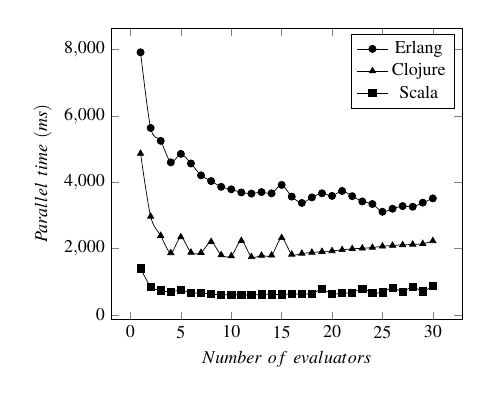
\begin{tikzpicture}[thick, scale=0.65]

  \begin{axis}[
         xlabel=$Number \hspace{.12cm} of \hspace{.12cm} evaluators$,
         ylabel=$Parallel \hspace{.12cm} time \hspace{.12cm} (ms)$
         ]
     \addplot[smooth,mark=*]  plot coordinates{
(1,7919.428571428572)
(2,5638.0)
(3,5249.75)
(4,4601.5)
(5,4856.714285714285)
(6,4567.285714285715)
(7,4208.333333333333)
(8,4036.0)
(9,3862.777777777778)
(10,3788.3)
(11,3693.6)
(12,3659.2)
(13,3705.1111111111113)
(14,3667.0)
(15,3920.4)
(16,3568.2)
(17,3376.75)
(18,3544.7)
(19,3668.222222222222)
(20,3589.4)
(21,3739.222222222222)
(22,3580.9)
(23,3421.6)
(24,3345.222222222222)
(25,3110.8)
(26,3202.4)
(27,3282.1)
(28,3262.0)
(29,3385.4)
(30,3513.777777777778)
     };
     \addlegendentry{Erlang}

     \addplot[smooth,mark=triangle*]
         plot coordinates{
         (1,4866.5)
(2,2970.0)
(3,2389.5555555555557)
(4,1870.5555555555557)
(5,2347.1111111111113)
(6,1882.888888888889)
(7,1878.111111111111)
(8,2206.1111111111113)
(9,1808.4444444444443)
(10,1777.3333333333333)
(11,2238.1111111111113)
(12,1752.3333333333333)
(13,1791.888888888889)
(14,1798.888888888889)
(15,2324.777777777778)
(16,1825.7777777777778)
(17,1854.5555555555557)
(18,1881.5555555555557)
(19,1908.6666666666667)
(20,1931.5555555555557)
(21,1962.888888888889)
(22,1993.6666666666667)
(23,2010.111111111111)
(24,2030.5555555555557)
(25,2071.0)
(26,2094.3333333333335)
(27,2112.8888888888887)
(28,2126.4444444444443)
(29,2144.5555555555557)
(30,2233.222222222222)
         };
     \addlegendentry{Clojure}


     \addplot[smooth,mark=square*]
         plot coordinates{
(1,1406.8333333333333)
(2,854.5714285714286)
(3,741.0)
(4,694.75)
(5,752.2)
(6,660.1111111111111)
(7,663.4285714285714)
(8,626.5)
(9,605.375)
(10,609.125)
(11,602.7777777777778)
(12,596.1428571428571)
(13,620.8888888888889)
(14,619.7777777777778)
(15,619.0)
(16,634.2222222222222)
(17,631.8888888888889)
(18,641.8888888888889)
(19,775.5555555555555)
(20,630.625)
(21,656.6666666666666)
(22,672.7777777777778)
(23,796.2222222222222)
(24,671.1111111111111)
(25,679.3333333333334)
(26,825.8888888888889)
(27,696.2222222222222)
(28,854.5)
(29,711.0)
(30,882.6666666666666)
         };
     \addlegendentry{Scala}

  \end{axis}

\end{tikzpicture}


%\textbf{Fig. 2.} Parallel running times for two reproducers and 0..30 evaluators of hybrid pGAs implementation in Erlang, Scala and Clojure.
%
%\end{itemize}
%\end{small}

\begin{small}


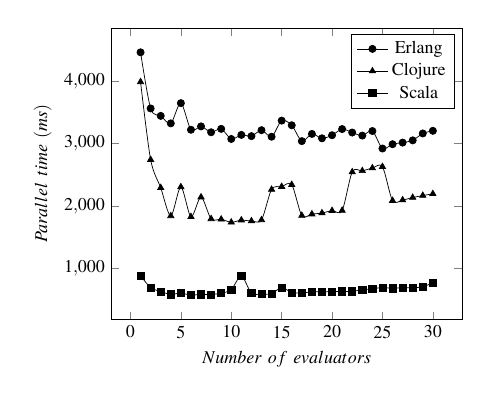
\begin{tikzpicture}[thick, scale=0.65]

  \begin{axis}[
         xlabel=$Number \hspace{.12cm} of \hspace{.12cm} evaluators$,
         ylabel=$Parallel \hspace{.12cm} time \hspace{.12cm} (ms)$
         ]
     \addplot[smooth,mark=*]  plot coordinates{
(1,4466.6)
(2,3564.222222222222)
(3,3444.6666666666665)
(4,3324.5555555555557)
(5,3649.6)
(6,3221.7)
(7,3275.9)
(8,3181.3)
(9,3236.0)
(10,3073.5555555555557)
(11,3139.0)
(12,3119.1111111111113)
(13,3214.9)
(14,3109.5555555555557)
(15,3368.3)
(16,3293.7)
(17,3039.1)
(18,3154.7)
(19,3084.1)
(20,3133.6666666666665)
(21,3232.9)
(22,3177.1111111111113)
(23,3128.0)
(24,3201.3333333333335)
(25,2920.4)
(26,2989.5555555555557)
(27,3015.4)
(28,3051.4444444444443)
(29,3162.3)
(30,3204.7)
     };
     \addlegendentry{Erlang}

     \addplot[smooth,mark=triangle*]
         plot coordinates{
(1,3990.75)
(2,2740.777777777778)
(3,2289.1111111111113)
(4,1837.111111111111)
(5,2302.5555555555557)
(6,1822.6666666666667)
(7,2138.6666666666665)
(8,1789.5)
(9,1782.3333333333333)
(10,1734.6666666666667)
(11,1768.888888888889)
(12,1754.7777777777778)
(13,1772.0)
(14,2261.1111111111113)
(15,2307.8888888888887)
(16,2338.4444444444443)
(17,1842.3333333333333)
(18,1865.7777777777778)
(19,1883.4444444444443)
(20,1920.7777777777778)
(21,1923.5)
(22,2542.1111111111113)
(23,2561.6666666666665)
(24,2605.5555555555557)
(25,2627.0)
(26,2083.0)
(27,2091.8888888888887)
(28,2132.222222222222)
(29,2163.777777777778)
(30,2192.1111111111113)
         };
     \addlegendentry{Clojure}


     \addplot[smooth,mark=square*]
         plot coordinates{
(1,876.6666666666666)
(2,683.7777777777778)
(3,622.2857142857143)
(4,575.2222222222222)
(5,596.0)
(6,563.0)
(7,576.2222222222222)
(8,574.0)
(9,595.1111111111111)
(10,651.8888888888889)
(11,871.6666666666666)
(12,595.3333333333334)
(13,582.25)
(14,586.8888888888889)
(15,684.8888888888889)
(16,605.0)
(17,600.625)
(18,614.0)
(19,618.2222222222222)
(20,616.7777777777778)
(21,625.2222222222222)
(22,622.6666666666666)
(23,649.7777777777778)
(24,664.1111111111111)
(25,686.625)
(26,672.4444444444445)
(27,684.7777777777778)
(28,681.625)
(29,698.0)
(30,760.7142857142857)
         };
     \addlegendentry{Scala}

  \end{axis}

\end{tikzpicture}


\textbf{Fig. 1.} Parallel running times for one reproducer and 0..30 evaluators of hybrid pGAs implementation in Erlang, Scala and Clojure.

\end{small}


\begin{small}


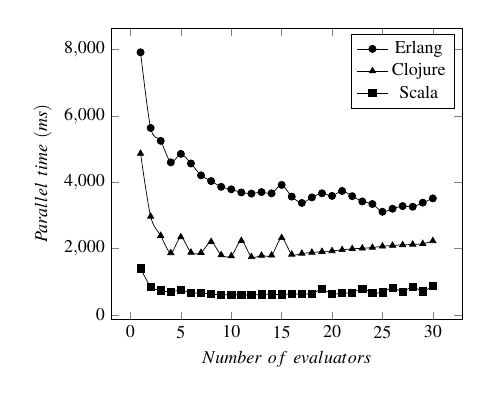
\begin{tikzpicture}[thick, scale=0.65]

  \begin{axis}[
         xlabel=$Number \hspace{.12cm} of \hspace{.12cm} evaluators$,
         ylabel=$Parallel \hspace{.12cm} time \hspace{.12cm} (ms)$
         ]
     \addplot[smooth,mark=*]  plot coordinates{
(1,7919.428571428572)
(2,5638.0)
(3,5249.75)
(4,4601.5)
(5,4856.714285714285)
(6,4567.285714285715)
(7,4208.333333333333)
(8,4036.0)
(9,3862.777777777778)
(10,3788.3)
(11,3693.6)
(12,3659.2)
(13,3705.1111111111113)
(14,3667.0)
(15,3920.4)
(16,3568.2)
(17,3376.75)
(18,3544.7)
(19,3668.222222222222)
(20,3589.4)
(21,3739.222222222222)
(22,3580.9)
(23,3421.6)
(24,3345.222222222222)
(25,3110.8)
(26,3202.4)
(27,3282.1)
(28,3262.0)
(29,3385.4)
(30,3513.777777777778)
     };
     \addlegendentry{Erlang}

     \addplot[smooth,mark=triangle*]
         plot coordinates{
         (1,4866.5)
(2,2970.0)
(3,2389.5555555555557)
(4,1870.5555555555557)
(5,2347.1111111111113)
(6,1882.888888888889)
(7,1878.111111111111)
(8,2206.1111111111113)
(9,1808.4444444444443)
(10,1777.3333333333333)
(11,2238.1111111111113)
(12,1752.3333333333333)
(13,1791.888888888889)
(14,1798.888888888889)
(15,2324.777777777778)
(16,1825.7777777777778)
(17,1854.5555555555557)
(18,1881.5555555555557)
(19,1908.6666666666667)
(20,1931.5555555555557)
(21,1962.888888888889)
(22,1993.6666666666667)
(23,2010.111111111111)
(24,2030.5555555555557)
(25,2071.0)
(26,2094.3333333333335)
(27,2112.8888888888887)
(28,2126.4444444444443)
(29,2144.5555555555557)
(30,2233.222222222222)
         };
     \addlegendentry{Clojure}


     \addplot[smooth,mark=square*]
         plot coordinates{
(1,1406.8333333333333)
(2,854.5714285714286)
(3,741.0)
(4,694.75)
(5,752.2)
(6,660.1111111111111)
(7,663.4285714285714)
(8,626.5)
(9,605.375)
(10,609.125)
(11,602.7777777777778)
(12,596.1428571428571)
(13,620.8888888888889)
(14,619.7777777777778)
(15,619.0)
(16,634.2222222222222)
(17,631.8888888888889)
(18,641.8888888888889)
(19,775.5555555555555)
(20,630.625)
(21,656.6666666666666)
(22,672.7777777777778)
(23,796.2222222222222)
(24,671.1111111111111)
(25,679.3333333333334)
(26,825.8888888888889)
(27,696.2222222222222)
(28,854.5)
(29,711.0)
(30,882.6666666666666)
         };
     \addlegendentry{Scala}

  \end{axis}

\end{tikzpicture}


\textbf{Fig. 2.} Parallel running times for two reproducers and 0..30 evaluators of hybrid pGAs implementation in Erlang, Scala and Clojure.

\end{small}


% \begin{multicols}{2}
% \begin{small}
% \begin{itemize}
% \item[] \textbf{Fig. 3.} Number of evaluators with best results for one reproducer.
%     
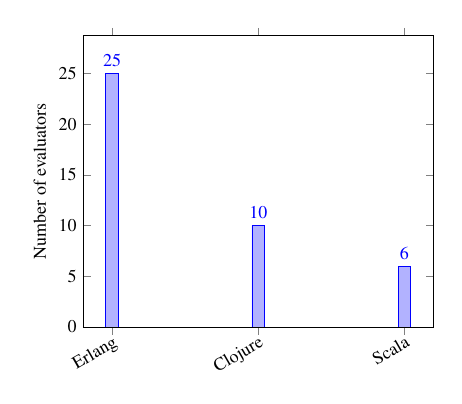
\begin{tikzpicture}[thick, scale=0.65]
  \begin{axis}[ybar,
    bar width=0.25cm,
    ymin=0,
    enlarge y limits={upper,value=0.15},
    legend style={at={(0.5,-0.25)},
    anchor=north,legend columns=-1},
    ylabel={Number of evaluators},
    symbolic x coords={Erlang, Clojure, Scala},
    xtick=data,
    xticklabel style={
        inner sep=0pt,
        anchor=north east,
        rotate=30
    },
    nodes near coords={\pgfmathprintnumber[fixed,precision=0]{\pgfplotspointmeta}},
    ]
    \addplot coordinates {(Erlang,25) (Clojure,10) (Scala,6)};
  \end{axis}
\end{tikzpicture}

% \columnbreak
% \item[] \textbf{Fig. 4.} Number of evaluators with best results for two reproducers.
%     
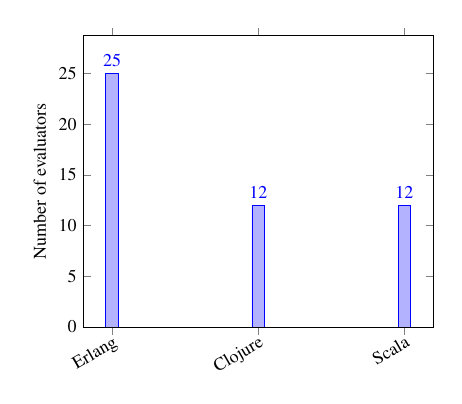
\begin{tikzpicture}[thick, scale=0.65]
  \begin{axis}[ybar,
    bar width=0.25cm,
    ymin=0,
    enlarge y limits={upper,value=0.15},
    legend style={at={(0.5,-0.25)},
    anchor=north,legend columns=-1},
    ylabel={Number of evaluators},
    symbolic x coords={Erlang, Clojure, Scala},
    xtick=data,
    xticklabel style={
        inner sep=0pt,
        anchor=north east,
        rotate=30
    },
    nodes near coords={\pgfmathprintnumber[fixed,precision=0]{\pgfplotspointmeta}},
    ]
    \addplot coordinates {(Erlang,25) (Clojure,12) (Scala,12)};
  \end{axis}
\end{tikzpicture}

% \end{itemize}
% \end{small}
% \end{multicols}

%\begin{small}
%\begin{itemize}
%\item[] \textbf{Fig. 3.} Parallel time for 25 evaluators (Erlang's best case).
%    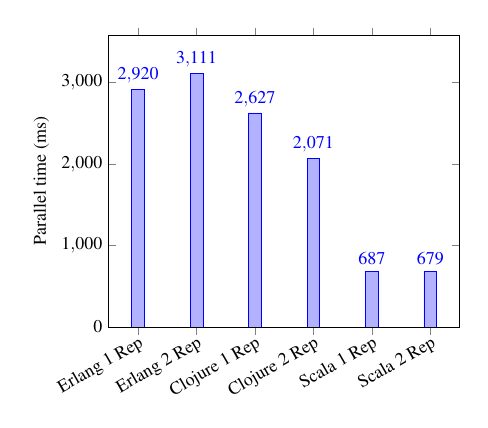
\begin{tikzpicture}[thick, scale=0.65]
  \begin{axis}[ybar,
    bar width=0.25cm,
    ymin=0,
    enlarge y limits={upper,value=0.15},
    legend style={at={(0.5,-0.25)},
    anchor=north,legend columns=-1},
    ylabel={Parallel time (ms)},
    symbolic x coords={Erlang 1 Rep, Erlang 2 Rep, Clojure 1 Rep, Clojure 2 Rep, Scala 1 Rep, Scala 2 Rep},
    xtick=data,
    xticklabel style={
        inner sep=0pt,
        anchor=north east,
        rotate=30
    },
    nodes near coords={\pgfmathprintnumber[fixed,precision=0]{\pgfplotspointmeta}},
    ]
    \addplot coordinates {(Erlang 1 Rep,2920.4) (Erlang 2 Rep,3110.8) (Clojure 1 Rep,2627) (Clojure 2 Rep,2071) (Scala 1 Rep,686.625) (Scala 2 Rep,679.3333333)};
  \end{axis}
\end{tikzpicture}
%
%
%\item[] \textbf{Fig. 4.} Parallel time for 10 evaluators (Clojure's best case).
%    
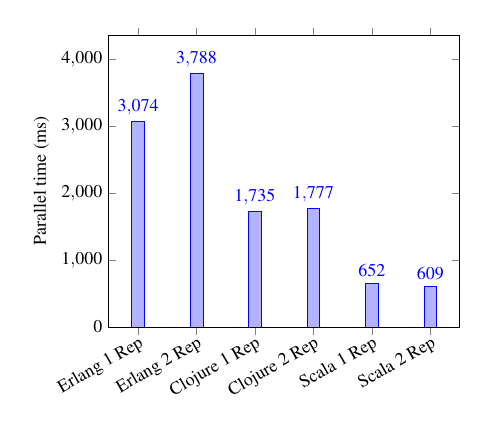
\begin{tikzpicture}[thick, scale=0.65]
  \begin{axis}[ybar,
    bar width=0.25cm,
    ymin=0,
    enlarge y limits={upper,value=0.15},
    legend style={at={(0.5,-0.25)},
    anchor=north,legend columns=-1},
    ylabel={Parallel time (ms)},
    symbolic x coords={Erlang 1 Rep, Erlang 2 Rep, Clojure 1 Rep, Clojure 2 Rep, Scala 1 Rep, Scala 2 Rep},
    xtick=data,
    xticklabel style={
        inner sep=0pt,
        anchor=north east,
        rotate=30
    },
    nodes near coords={\pgfmathprintnumber[fixed,precision=0]{\pgfplotspointmeta}},
    ]
    \addplot coordinates {(Erlang 1 Rep,3073.555556) (Erlang 2 Rep,3788.3) (Clojure 1 Rep,1734.666667) (Clojure 2 Rep,1777.333333) (Scala 1 Rep,651.8888889) (Scala 2 Rep,609.125)};
  \end{axis}
\end{tikzpicture}
%
%\end{itemize}
%\end{small}

Figures 1 and 2 show that the three languages have a good concurrent behaviour: the overhead of managing more logical execution units than the available physical ones did not show any impact on the execution time of the algorithm, even when that number gradually increases.

%\setcounter{figure}{4}
%
%\begin{figure}
%\caption{Parallel time for 6 evaluators (Scala's best case).}
%\centering
%    
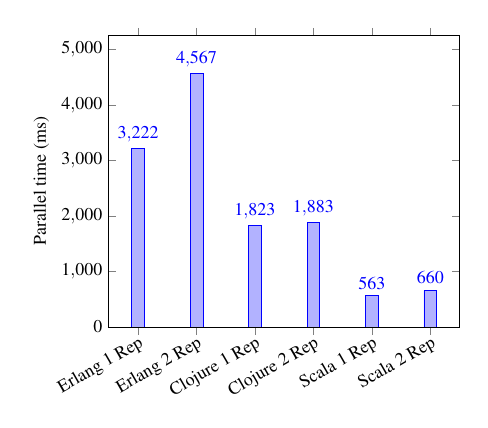
\begin{tikzpicture}[thick, scale=0.65]
  \begin{axis}[ybar,
    bar width=0.25cm,
    ymin=0,
    enlarge y limits={upper,value=0.15},
    legend style={at={(0.5,-0.25)},
    anchor=north,legend columns=-1},
    ylabel={Parallel time (ms)},
    symbolic x coords={Erlang 1 Rep, Erlang 2 Rep, Clojure 1 Rep, Clojure 2 Rep, Scala 1 Rep, Scala 2 Rep},
    xtick=data,
    xticklabel style={
        inner sep=0pt,
        anchor=north east,
        rotate=30
    },
    nodes near coords={\pgfmathprintnumber[fixed,precision=0]{\pgfplotspointmeta}},
    ]
    \addplot coordinates {(Erlang 1 Rep,3221.7) (Erlang 2 Rep,4567.285714) (Clojure 1 Rep,1822.666667) (Clojure 2 Rep,1882.888889) (Scala 1 Rep,563) (Scala 2 Rep,660.1111111)};
  \end{axis}
\end{tikzpicture}
%\end{figure}

The Scala implementation is smoother in its results in contrast with
Clojure where many peaks were obtained.
These two languages use the JVM and the same random library, however there are clear differences in their concurrent models. The results for Scala and Clojure are better with a small number of units of execution: when the number of evaluators grows the efficiency of the algorithm falls. In this sense Erlang have a non-typical behaviour, improving up to 25 evaluators, and then the speed begins to decrease.

Erlang is the language with the worst execution time; but its runtime, in the best case, is able to schedule 52 units of execution (far more than the others). The Erlang processes are scheduled using SMP whith one scheduler per core. Each process is allowed to run until it is paused to wait for input (a message from some other processes) or until it has executed a maximum fixed number of reductions (each VM instruction has associated a number of reductions). This unique way of scheduling processes yields these particular results and will be better used in next studies. Also the speedup obtained in relationship with his sequential time is very good. These two facts point to a possible good scalability.

Clojure's performance is medium, with a speedup close to $1$. The {\em send} function was always used to compute the expression by the agents therefore a hardware dependent pool of treats was used.

Scala is the language with best results, even when its runtime is the same of Clojure's. It has a particular model of concurrency (actors on a {\em event-based} dispatcher supported on the Java JSR166 fork-join pool); and of computation (its balance between mutable and immutable state), allowing the best behaviour of the concurrent algorithm. Again is important to note the quality of the concurrent abstractions made by all these technologies in which the number of logical units of executions is greater than the number of the physical ones.



\subsection{Sample Program of Canonical Island/GA in Scala}\label{sec:sample}
In order to highlight the simplicity of the code based in the built in concurrent concepts of the selected languages. We will describe a canonical island-based GA implementation in Scala. We take and island-based GA implementation because is simpler parallel GA model than  hybrid pGAs we use for time evaluations.

Scala inherit keywords from several languages to express programming concepts: from Java take {\em extends} for express inheritance and from Python/Ruby take {\em def} to define methods. In order to help the type inference they have Pascal-like syntax for declaring types.

The listing \ref{island} shows a class declaration: an actor class.

\lstset{language=scala, captionpos=b, caption={Actor declaration.},label=island, basicstyle=\ttfamily\footnotesize}
\begin{lstlisting}[frame=none]
class Island extends Actor {
  // Set of actors (workers)
  var workers: Set[ActorRef] = _
  def receive = {
     case 'start =>
      // All executing units to work!
      workers.forEach(_ ! 'start)
  }
}
\end{lstlisting}

{\em Island} is an {\em actor}, it have a set of others actors (the workers reproducers and evaluators). All actors classes should have a {\em receive} method, this block of code is compound of a list of case instructions: one for each kind of message the actor is able to respond. In this method there is only one case: for send a {\em 'start} message to each worker. All actors have a method of name {\em !} to send messages to them.

\lstset{language=scala,captionpos=b, caption={Functional processing of data.},label=reproducer}
\begin{lstlisting}[frame=none]
// One of the worker classes
class Reproducer extends Actor {
  def receive = {
    case ('evolve, pool:HashMap, n:Int)
             =>
    val pop = pool.filter((a: (List,
            (Int, Int))) => a._2._2==2).
            keys.toList.map(i =>
                         (i, pool(i)._1))
      val (res, resultData) =
        Reproducer.evolve(
        Reproducer.extractSubpop(pop,n),
          parentsCount = n / 2 })
        // Continue the iteration with
        // res and resultData
 }
}
\end{lstlisting}

The listing \ref{reproducer} shows the class for the reproducers, in this case the message processed is composed of a tuple of 3 elements. The first statement apply a filter and a transformation (method {\em map}) over the pool of individuals.

\lstset{language=scala,captionpos=b, caption={Main code.},label=main}
\begin{lstlisting}[frame=none]
// Creating 4 islands
val islands = for(_ <- 1 to 4)
       yield sys.actorOf(Props[Island])
		
// Puting the migrants destination & start
// each island
for(i <- 0 to 3){
	islands(i) ! ('migrantsDest,
	              islands((i+1)%4))
	islands(i) ! 'start
}
\end{lstlisting}

Finally the listing \ref{main} create islands and start the evolutions.  

\section{\uppercase{Conclusions}}
\label{sec:conclusions}
    
This work shows the implementation simplicity of a hybrid parallel genetic algorithm in functional-concurrent languages. The executions units was map to build-in concurrent concepts of languages (actors and agents) and the procedurals to functions or methods.

The GA model used had a shared memory data structure and the less pure language (Scala) had advantages and got the bests results.

%¿Qué es lo que está comentado? La conclusión es un poco corta... La segunda frase no tiene sentido.


%En el modelo implementado es necesario compartir memoria (el pool) de manera intensa. Scala al ser un lenguaje híbrido que combina los paradigmas OO y funcional, y por lo tanto los modelos de cómputo con cambios de estado (imperativo, procedural) y los sin cambio de estado (declarativo, funcional) presenta ante los demás una clara ventaja que se ve reflejada en los resultados numéricos. Tanto en las versiones secuenciales como en las concurrentes este lenguaje fue el mejor, concluyéndose que en modelos de AGs como este Scala es el más adecuado.

%The GA model used require sharing memory (the pool) among executing units. Scala is



%\section{Acknowledgements}
%
%This work is supported by projects TIN2011-28627-C04-02 (ANYSELF),
%awarded by the Spanish MINECO and CANUBE (CEI2013-P-14) awarded by CEI
%BioTIC, as well as MUSES (http://musesproject.eu) awarded by the
%European commission. It is also supported too by the PhD
%Program of the AUIP.


%\bibliographystyle{splncs}
%\bibliography{osgiliath,geneura,referencias,erlang-ae-model}

\vfill
\bibliographystyle{apalike}
{\small
\bibliography{osgiliath,geneura,referencias,erlang-ae-model}}

\end{document}

